
\chapter[Approach]{Approach}
\graphicspath{ {images/approach} }

Comprehending the evolution of a software system is a complex activity, mainly because of the sheer amount of data and its complexity. 
The term "software evolution" was coined for the first time by Lehman in 1985 in a set of laws. \cite{Lehman1985}
He stated that the complexity of a system is destinated to increase over time, as the system always needs to be adapted to its evolutionary environments. 
To be managed, software systems need to be comprehended by developers, and this activity can be simplified with software visualization. 

Over the last ten years, developers have stored their codebase on git repositories. 
For this reason, we focused our attention on systems versioned with this protocol.

Git is a versioning control system that tracks all the changes made to every system file. 
Internally git holds all the information that we need to reconstruct the history of a repository. 

In this chapter, we present our approach for visualizing a software system using a visual and auditive depiction of the evolution of a system. 
To fulfill this purpose, we have chosen to leverage the phenomenon of Synesthesia, the production of a sense impression relating to one sense by stimulation of another sense.
Moreover, we also present how we reconstruct and model the history of a repository. 

Our approach is composed of three parts: 
\begin{itemize}
    \item in the first section, we model the evolution of a system; 
    \item in the second section, we present two ways to visualize the system 
    \item in the third section, we show how music can be used to communicate evolutionary information. 
\end{itemize}


\section{Evolution Model}
\label{s:EvolutionModel}

\begin{figure}[H]
    \begin{center}
        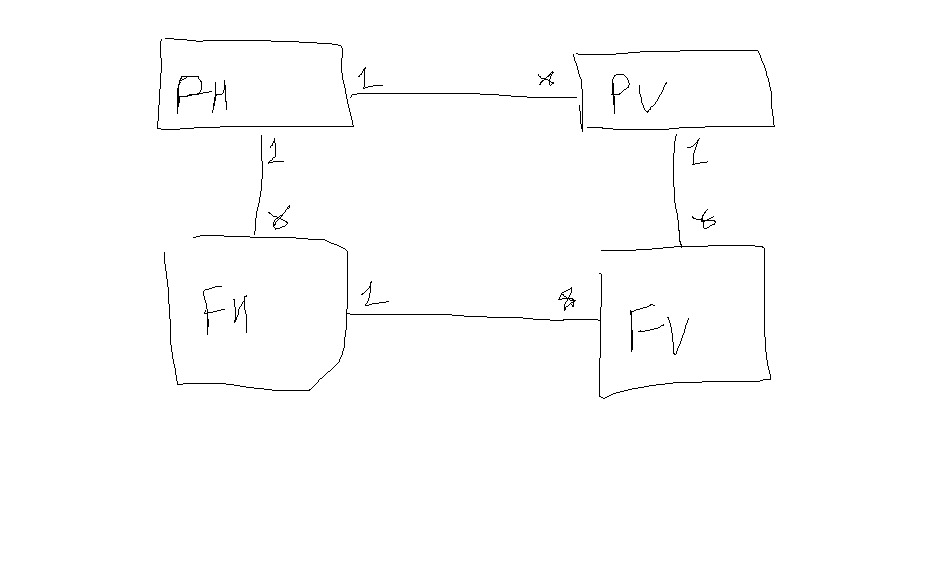
\includegraphics[width=0.6\textwidth]{EvolutionaryModel.jpg}
    \end{center}
    \caption{Evolutionary Model}
    \label{fig:EvolutionaryModel}
\end{figure}

To model the evolution of software systems, we developed the model 
shown in figure \ref{fig:EvolutionaryModel}. It is based on Hismo, a solution presented by Tudor Girba \cite{Girba2005}.\\
\\
The need to develop a novel evolutionary model comes from the fact that Hismo was designed to work with another versioning system: Subversion (SVN). 
There are several differences between SVN and git. In terms of design, the most important is how they keep track of changes. 
SVN works with the concept of "snapshot" while git works with the concept of "commits".
In SVN, when a file has been changed, a new revision of the whole system is created, and consequently, the number of revisions is incremented. 
In contrast, in git, only the modified files would get committed, and thus we don't have every time a new snapshot of the system. 
Therefore, we took Hismo as the starting point of our model and we adapted it to make it work with the git protocol. 
Initially, the Hismo model was based on three concepts:
\begin{itemize}
    \item Snapshot. A representation of the entity whose evolution is studied.
    \item Version. An entity that adds the notion of time to a Snapshot by relating it to History. 
    \item History. An entity that holds a set of Versions.
\end{itemize}


Git does not have the concept of Snapshot, so we replaced it with a novel concept: FileVersion. 
A FileVersion is essentially the version of a file at a particular point in time. 
It has the same fashion as a Snapshot. Still, instead of being related to every version of the system, it is related only to the Versions where the file was effectively updated.
Moreover, we made a distinction between File entities and Project entities. So, we mapped the concept of History to FileHistory and the idea of Version to ProjectVersion. 
The entity responsible for holding both of them is called ProjectHistory. 
To summarize, these are the four main concepts of our model: 
\begin{itemize}
    \item \textbf{ProjectHistory}: represents the history of a repository. It is the holder of two sets: a set of FileHistories and a set of ProjectVersions. 
    \item \textbf{FileHistory}: represents a file of the repository. We consider each file as an entity of the system. Even if the entity's name or location is changed, our mode will treat it as the same. So, our approach is resilient to renaming and moving activities. Each FileHistory holds a set of FileVersion, each one representing a different version of the entity at a particular point in time.  
    \item \textbf{ProjectVersion}: represents a commit or a version of the system. 
    For each changed file inside a commit, the respective ProjectVersion contains a FileVersion representing that change.
    A ProjectVersion also holds contextual information about the commit, such as the timestamp, the hash of the commit, and the message.
    \item \textbf{FileVersion}: represents the version of an entity at a particular point in time.
    It is responsible for holding all evolutionary information of an entity since it represents an evolutionary step of that entity. 
\end{itemize}

\subsection*{Historical information retrival}
To build the history of a repository, we need to extract the historical information from git.\\

To understand better how we approached it, we have to explain how git internally represents the repository history. 
Git works with the concept of branches; each branch can be seen as a different repository timeline.
Usually, developers exploit branches to develop features on them and then merge the developed code in a branch that contains the stable codebase.
They need to create a "merge commit" to do that. 
Each time we create a new git commit, we deploy a new version of the system that records all the changes made to the commits' tracked files. 
Internally, in git, all the commits are stored as nodes of a commit-tree. 
The root node represents the repository's first commit since it has no parents. 
All the other nodes instead represent the commits made during the whole lifecycle of the repository. 
Each commit usually has only one parent, representing the previous commit made before that one.
There is one case where a commit might have more than one parent: merges commits.

Each repository should have a branch containing stable, production-ready code, as a convention. Usually, this branch is named "main" or "master". 
In our approach, we aim to analyze the timeline of this stable branch. We start from the root of the commit tree, which represents the initial commit, and then we traverse the whole tree. 
However, we don't consider "merge commits" during this process since they already incorporate commits previously made, and thus they would be considered twice. 
Once we have extracted all the valid commits that reside on the stable branch, we need to take from them all the representative information that we need to represent a ProjetctVersion. \\

Git can recognize the following actions made on a file:
\begin{itemize}
    \item \textbf{ADD}. A file is added to the repository.
    \item \textbf{DELETE}. A file has been removed from the repository.
    \item \textbf{MODIFY}. A file has been modified.
    \item \textbf{RENAME}. A file's name has been changed. Whether the file path has been changed, the parent directory path must remain the same. 
    \item \textbf{MOVE}. A file was moved from one location to another, so the file path changed. This action id detected whether the filename remains the same. 
\end{itemize}

From a commit, we could also extract additional information such as the name of the file being modified, the action made on a file, the number of lines added and removed, the path of the file before and after the changes, and many more.
We used the commit's information to track all the paths of an entity. Therefore, we can update the entity path when it was renamed or moved to follow it during its lifecycle. \\
%\linebreak
When we reconstruct the history of a repository, each FileHistory starts with a FileVersion representing an ADD action. Then, in the middle of the FileVersion set, we can find only three kinds of actions: MODIFY, RENAME, and MOVE. 
During the lifecycle of a repository, sometimes, files are deleted; in this case, the last FileVersion held by a deleted FileHistory represents a DELETE action.

\begin{figure}
    \begin{center}
        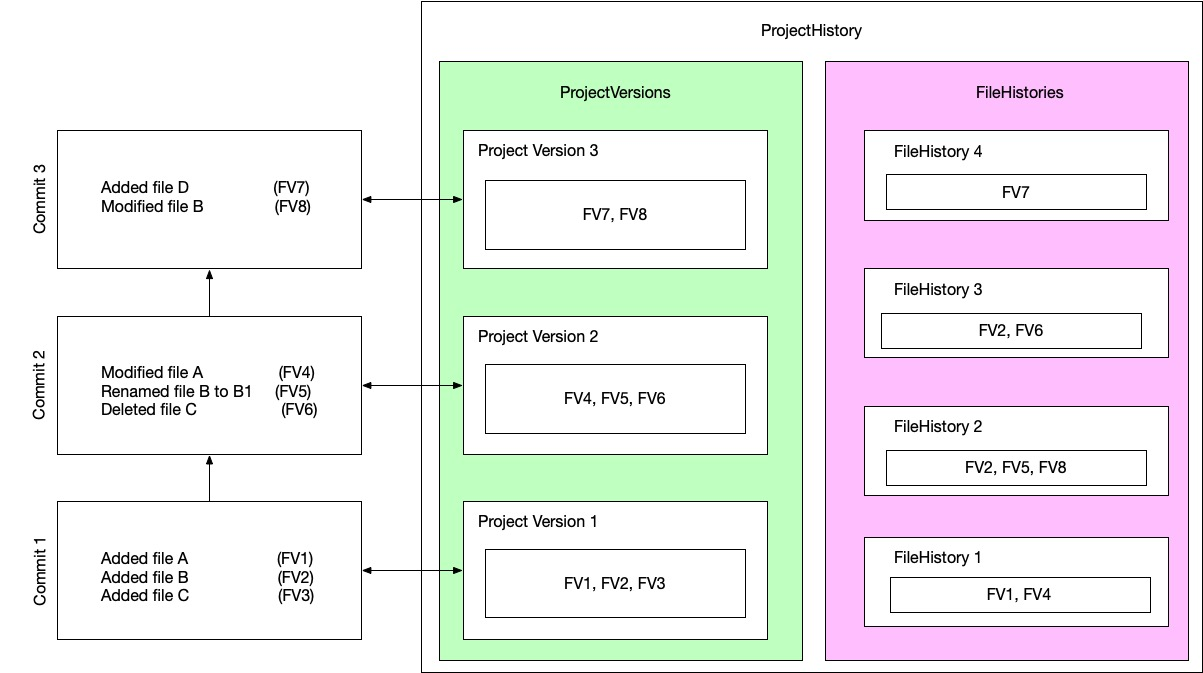
\includegraphics[width=0.8\textwidth]{RebuildingHistory.jpg}
    \end{center}
    \caption{Rebuilding history example}
    \label{fig:RebuildingHistory}
\end{figure}

\autoref{fig:RebuildingHistory} shows an example of how history is rebuilt.
First, we create a ProjectHistory with a set of ProjectVersions and a set of FileHistories.
After that, we start to traverse the repository's commit tree.
As we can notice, for each commit, we create a new ProjectVersion. For us, it represents a new version of the system. 
Therefore, we inspect the commit's changelog and create a new ProjectVersion for each list entry.
In this way, every time we encour an added file into the changelog, we create a new FileHistory. 
At version 1, three new files were added to the repository (A, B, C), and, as we can see, three new FileHistories were created.
Each change was mapped to a FileVersion (FV) and consequently added to the respective FileHistory and ProjectVersion. 
We did the same thing for ProjectVersion 2 and 3. 

\label{s:partialHistoricalRepr}
\subsection*{Partial historical representation}
One of our goals, when we developed this approach, was the possibility of analyzing a large repository in an acceptable amount of time. 
In other words, our approach needs to be scalable.
GitHub host the code of some notorious open-source systems, such as LibreOffice, Elastisearch, and Linux.
They all have more than 500,000 commits in each, and thus, we cannot aim to reconstruct their histories with a single analyzer; it will take too much time.  
To prove that, just consider the worse case: Linux. 
When this thesis was redacted, the repository of Linux had 1,090,563 commits. 
To move from one commit to another, we could assume that git needs one second. 
As a result, just to navigate through the whole history of Linux, we would need 11 days.
Moreover, in this simple estimation, we are omitting the vast amount of time the analyzer needs to extract metrics from every single file on each version. 

We present a scalable approach based on the concept of partial history.
A partial history is an object that holds information about a specific range of time of the ProjectHistory. 
It can be seen as a subset of a ProjetHistory. 
We can split the repository's history into multiple parts, each represented by a partial record. Then when all the analyses are completed, we merge them to reconstruct the whole story of the repository.


\begin{figure}
    \begin{center}
        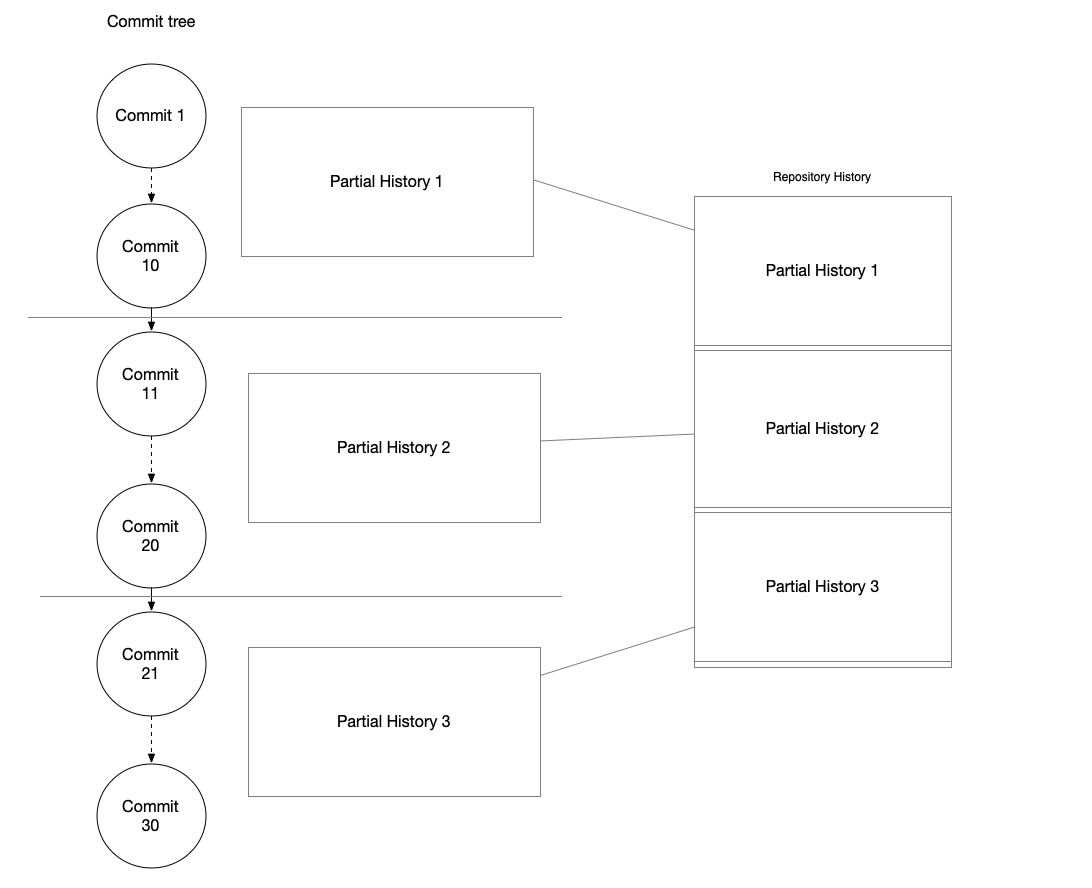
\includegraphics[width=0.6\textwidth]{PartialHistory.png}
    \end{center}
    \caption{Partial history example}
    \label{fig:PartialHistory}
\end{figure}

\autoref{fig:PartialHistory} shows an example of PartialHistory representation. 
We split the commit tree into multiple chunks, and then ran the analysis on each piece. 
This analysis can be done in parallel since these chunks are independent. 
In the end, the final history will be represented by merging all the PartialHistories. \\
\\
Nonetheless, we can build PartialHistories in parallel; we cannot do the same for the final History. 
The final merge needs to be done sequentially. The sequence needs to follow the order of the commit tree. 
In \autoref{fig:PartialHistory}, for example
PartialHistory1 represents the history from commit 1 to commit 10, 
PartialHistory2 represents the history from commit 11 to commit 20, and finally 
PartialHistory3 represents the history from commit 21 to commit 30.
Therefore, the commit order is respected if we merge them in this order: 1, 2, 3. 
\\
The result of a single analysis and a parallel analysis must be identical. 
To ensure that, we need to pay attention to the merge operations of our analysis.
When we merge the history of a repository with a partial history, we need to preserve the characteristics of our model. 
In particular, if FileHistory is already present in our history, we don't have to duplicate it, but instead, we need to update it. 

\label{s:evolutionaryMetrics}
\subsection*{Evolutionary metrics}
Every version of the system holds a set of files. 
As we said, each file is represented by a FileVersion, which is part of a FileHistory. 
To understand the differences among all the FileVersions of a FileHistory,
we decided to collect some metrics to represent the state of a file within a version.\\
\\
Since we aim to have a language-agnostic approach, we have selected only language-agnostic metrics. 
However, the set of metrics of this approach can be easily extended.
We have defined a taxonomy to classify and categorize all the files present in a system. 
Each category is then mapped to a set of metrics. Moreover, metrics can be inherited by parent categories. 
\autoref{fig:taxonomy} shows an example of a possible taxonomy definition. \autoref{table:metricsT} shows the final set of metrics associated with each FileType. For each FileType, we compute the metric SIZE since it is inherited from the root FileType of our taxonomy. Moreover, the Textual FileType defines a set of metrics inherited by the Java FileType. 
\\

\begin{figure}
    \centering
    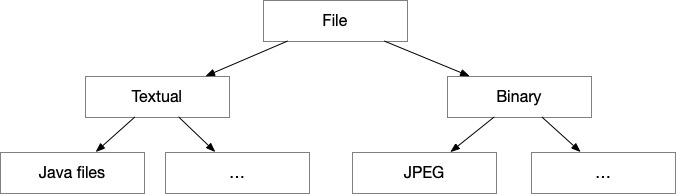
\includegraphics[width=0.6\textwidth]{Taxonomy.jpg}
    \caption{Taxonomy}
    \label{fig:taxonomy}
\end{figure}

\begin{table}[ht]
    \centering
    \begin{tabular}{lcr} \hline
        {\bf FileType} & {\bf Metrics}\\ \hline
        File    & SIZE      \\
        Textual & LOC, LinesAdded, LinesRemoved + SIZE \\
        Binary  & SIZE         \\
        Java    & SLOC + LOC, LinesAdded, LinesRemoved + SIZE \\
        JPEG    & SIZE \\
    \end{tabular}
    \caption{Example of metrics collected and inherited for each FileType}
    \label{table:metricsT}
\end{table}

We have defined a small set of metrics composed of the ones shown in \autoref{table:metricsT}. We are aware that this set is too small and, of course not perfect. However, our approach focuses not on the metrics collected but on how they are represented. Most importantly, any developer can easily extend our set of metrics.


\section{Visualization}
% The approach that we have defined can be applied to different contexts. 
We can represent a ProjectHistory with two kinds of visualization: a 2D visualization, which uses a matrix and works better with small systems, and a 3D visualization that can exploit human perception as a vector of information. 


\subsection{2D Representation}
This visualization is based on the Evolution Matrix approach defined by Lanza \cite{Lanza2001}. 

We said that a ProjectHistory is a holder of ProjectVersions and FileHistories. 
A ProjectVersion represents a commit of the system, whereas a FileHistory represents the history of a file. 
The connection between these two entities is a FileVersion that describes the state of a file in a system's version. \\
We can represent a ProjectHistory through a matrix with the following properties: 
\begin{itemize}
    \item Each column of the matrix represents ProjectVersion, a commit of the repository. 
    \item Each row of the matrix represents a FileHistory, the history of a file. 
    \item Each cell of the matrix represents a ProjectVersion, the state of a file at a specific point in time defined by the commit. 
\end{itemize}

Since we built our model on the top of git, we don't track snapshots of a system but only changes. 
An empty cell represents a FileHistory (row) that was not modified in a ProjectVersion (column). 
This concept was not present in the Evolution Matrix of Lanza because its model worked with SVN, and thus, it worked with the idea of incremental snapshots.  

\begin{figure}
    \center
    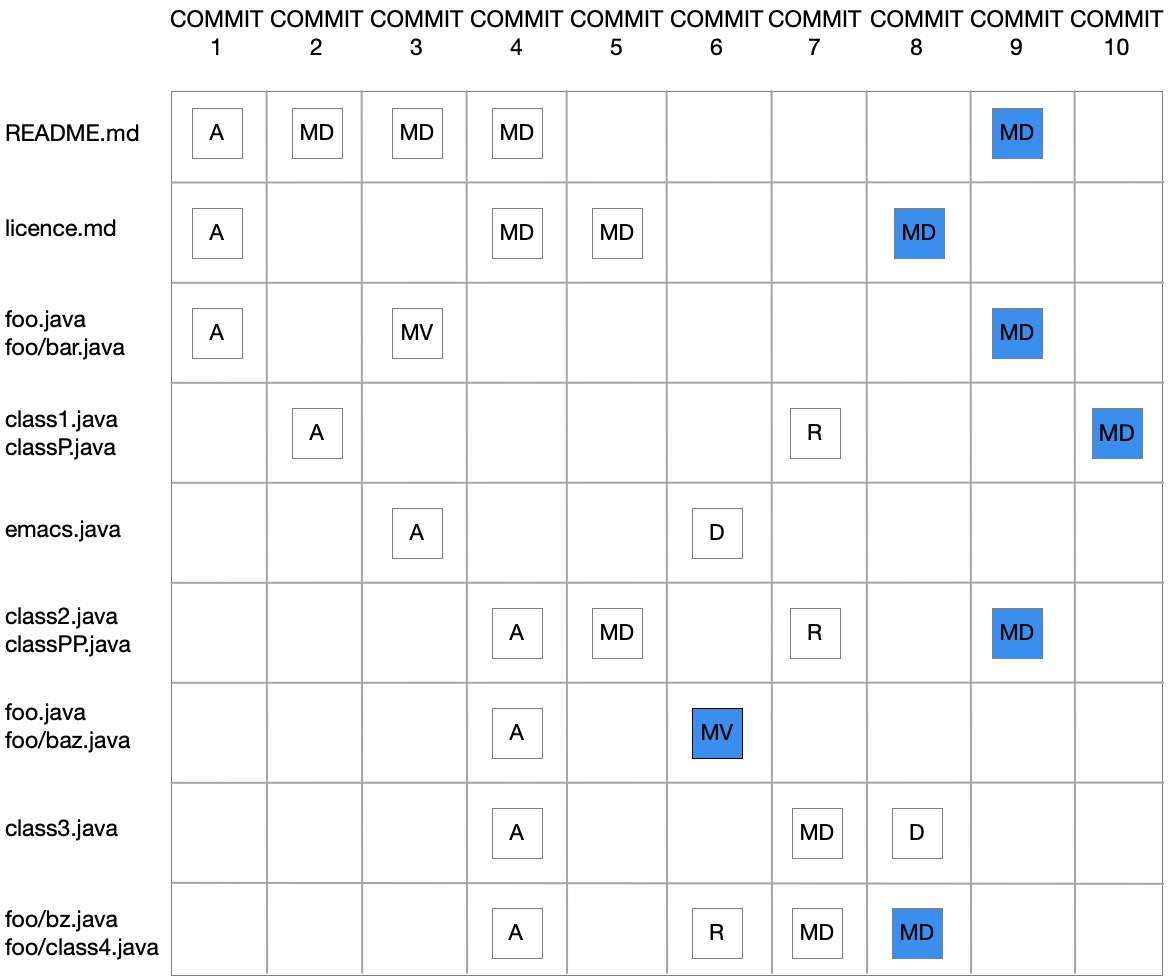
\includegraphics[width=0.6\textwidth]{2DMatrix.jpg}
    \caption{2D Representation of the structural evolution of a repository}
    \label{fig:evolutionMatrixApproach}
\end{figure}
\autoref{fig:evolutionMatrixApproach} depict the evolution of a repository with 14 files and 10 commits. In this figure we only show the structural evolution of a repository, without considering file's metrics as Lanza did. 
Each row represents the history of a file; therefore, it is associated with a set of FileVersions represented by the squares inside each cell. Actions made on a file are labeled as: A for ADD, M for MODIFY, MV for MOVE, R for RENAME, and D for DELETE.
As we can see, the first action made on each file is an ADD; moreover, some files end their history with a DELETE. It's essential to notice that \texttt{foo.java} and \texttt{foo/bar.java} are represented by the same FileHistory because they represent the same logical entity in the system. In fact, on commit 3 \texttt{foo.java} was moved into \texttt{foo/bar.java}. The same thing goes for \texttt{foo.java} and \texttt{foo/baz.java} represented by the seventh FileHistory.

Based on our aim, we can read this matrix as follows:
 \begin{itemize}
     \item \textbf{by rows}, if we are interested in the history of a particular entity of our system. 
     For example, the FileHistory represented by the first row in \autoref{fig:evolutionMatrixApproach} represents the history of \texttt{README.md}. 
     \texttt{README.md} was added in the first ProjectVersion (COMMIT 1) and then modified in the second, third, fourth, and ninth ProjectVersion.
     Moreover, \autoref{fig:evolutionMatrixApproach} is an excellent example to understand why we cannot rely only on the file name to identify a system's entity. 
     We can notice that \texttt{foo.java}, represented by the third FileHistory, was added with the first ProjectVersion and then moved with the third into \texttt{foo/bar.java}. 
     Then, on commit 4, a new file \texttt{foo.java} was added. Nonetheless, the name of the files are the same, they COMMIT two different entities. 
     \item \textbf{by columns}, if we are interested in which entities were updated on each ProjectVersion. 
    For example, on the first ProjectVersion, we have added the \texttt{README.me} file, the \texttt{licence.md} file and the \texttt{foo.java} file. 
 \end{itemize}

In addition, \autoref{fig:evolutionMatrixApproach} also provides an example of how we reconstruct the system's state after a commit. 
As we have seen, each ProjectVersion does not represent a system snapshot.
Instead, it represents only the difference in changes made to the previous version. 
To reconstruct the system's state at a specific version, we need to consider, for each FileHistory, the last change made before that version. 
Under those circumstances, for each FileHistory, we must go back in time until we find the rightmost change. Of course, if the rightmost difference was a DELETE, we must ignore the related FileHistory.
In \autoref{fig:evolutionMatrixApproach}, the state of the system after COMMIT 10 is composed of the FileHistories that hold a row with a blue square. 



\subsection{3D Representation}
\label{s:3DRepr}

Software systems are hard to understand due to the complexity and the sheer size of the data to be analyzed.
In our approach, we aim to make an interactive 3D representation to ease the comprehension task of the developer. 

Not all pieces of knowledge cannot be extracted by a metric or by a non-interactive graph. This is normal because both of them are responsible for representing only one piece of information simultaneously. For example, if we look at the graph of a repository code frequency, we can never understand which file was modified; because we have only two dimensions: the time and the code. The main advantage of our approach is the possibility of having multiple sources of information simultaneously. Our 3D representation aims to make system analysis easier for engineers by exploiting the human senses.
To do that, we have chosen to leverage the phenomenon of \textbf{synesthesia}. The phenomenon of synesthesia occurs when stimulation of a sense or a cognitive pathway leads to the involuntary stimulation of another reason or a cognitive path. We experience synesthesia when two or more things are perceived as the same. 
For example, synesthetic people might associate the red color with the letter D or the green color with the letter A. 
There are many forms of synesthesia, each one representing a different type of perception, such as visual forms, auditory, tactile, etc.

To visualize a project, we introduce the concept of \textbf{view}. We define a view as a way to illustrate the evolution of a project given a set of specifications. This set of specifications determines how the view must be built. For example, if we want to traverse the repository history by year, this information is part of the specification. A view holds a set of frames, called \textbf{AnimationFrame}, each representing the repository's whole state during a specific moment of its evolution. Therefore, the whole history of the repository is displayed by rendering these AnimationFrames consequently, like in a movie. 

Each repository has a unique history. There are young repositories whose history is 1 year long and old repositories with more than 10 years of development activity. It is not guaranteed that the number of commits is proportional to the age of a repository. Many repositories are dead on GitHub whereas others might have a vast amount of contributors rising the total number of commits every day. Therefore, we cannot provide a static approach to traverse the history of a repository. 
Every visualization has its own goal and its own way to traverse time. For this reason, we provide two visualization strategies to group commits into AnimationFrames. Both of them traverse the whole history from the beginning until the end.
\begin{itemize}
    \item{Grouping by commits}: the user specifies a number of commits \texttt{n} and then one AnimationFrame is created every \texttt{n} commits. With this strategy, the concept of time is lost because we consider only the position of the commit in the commit tree. Therefore development phases cannot be identified. 
    \item{Grouping by timestamp}: the user specifies a timestamp window \texttt{ts} and then one AnimationFrame is created every \texttt{ts} seconds. All the commits inside the time window are part of the AnimationFrame. Therefore, we might have empty AnimationFrames if in that time window were not made any commits. 
\end{itemize}

When an AnimationFrame is created, if multiple commits were made on a file, only the most recent one is considered. 
\autoref{fig:TimeWindowExamples} shows an example of three different strategies applied over the same history. As we can notice, in \autoref{fig:TimeWindow1} we made an AnimationFrame every 3 commits; as a result, the notion of time is lost. With a commit grouping strategy, we can never have an empty AnimationFrame. With  \autoref{fig:TimeWindow2} and \autoref{fig:TimeWindow3} the thing is different. Here we have empty AnimationFrames, and with these examples, we highlight the importance of a well-designed time window. Each project has its length of history. Therefore, with this example, we can underline our need to leave to the user the choice of the time window length. To avoid the case of a view with too many AnimationFrames, younger repositories might have a daily time window. In contrast, it might be better to have weekly, monthly, or yearly views for the older repository. 

In any case, if we pick two repositories born at the same time, the number of AnimationFrames is always the same because it does not depends upon the number of commits made. 


\begin{figure}
    \begin{center}
        \begin{subfigure}{1\textwidth}
            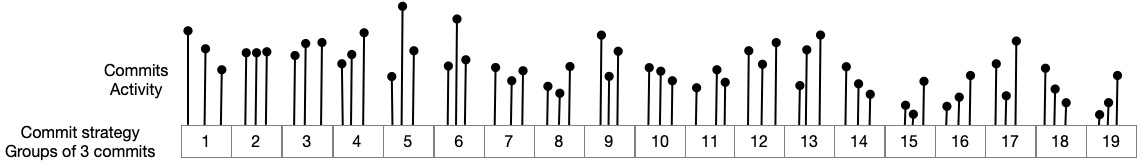
\includegraphics[width=\linewidth]{TimeWindow1.jpg}
            \caption{Grouping every 3 commits.} 
            \label{fig:TimeWindow1}
        \end{subfigure}
        \begin{subfigure}{1\textwidth}
            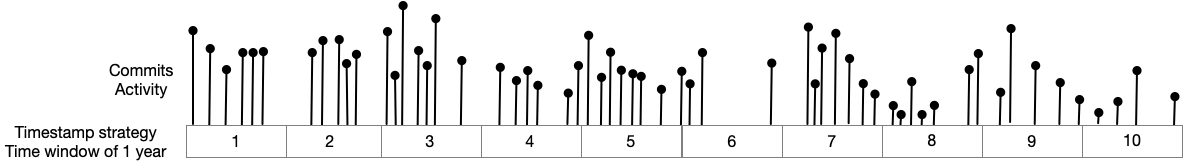
\includegraphics[width=\linewidth]{TimeWindow2.jpg}
            \caption{Grouping every year.} 
            \label{fig:TimeWindow2}
        \end{subfigure}
        \begin{subfigure}{1\textwidth}
            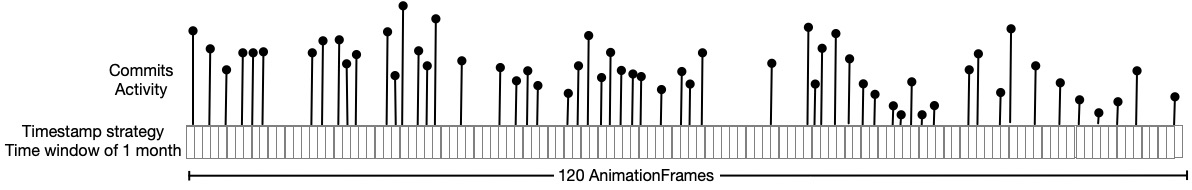
\includegraphics[width=\linewidth]{TimeWindow3.jpg}
            \caption{Grouping every month.}
            \label{fig:TimeWindow3}
        \end{subfigure}
        \caption[Example of three different grouping strategies]{Example of three different grouping strategies applied over a system whose history is 10 years long and it has 57 commits}
        \label{fig:TimeWindowExamples}
    \end{center}
\end{figure}



To represent the system's state, an AnimationFrame holds a set of \textbf{ViewFigure}, each representing a file part of the system.

A ViewFigure holds a set of properties used by the render process to draw a glyph representing a file. They represent abstract concepts; therefore, being understood by any 3D engine, anyone can reproduce our visualization approach. 

\subsection*{Layout}
Many tools have been proposed in the literature to depict the evolution of software with different layout strategies. 
One of the most famous approaches is the city metaphor \cite{Wettel2007}, presented by Lanza, where the file's position depends upon the package that holds it. 
Nonetheless, it works very well with small and medium systems; the interactivity and navigability can be substantially slowed down with large systems.

Therefore, our visualization strategy's main goals are scalability and incrementality. The visualization needs to scale, even with a very large repository, and it must visualize the system's evolution incrementally. Therefore, the user can immediately distinguish older entities from newer ones.

Under those circumstances, we adopted a spiral layout with an outward direction. Older entities are positioned at the center of this spiral, whereas newer entities are always close to borders. 
\autoref{fig:layout} shows an example of how ViewFigure is laid out with an outward spiral layout.

Hence, each ViewFigure has a \textit{position} to describe its position inside the 3D environment. 

\begin{figure}
    \center
    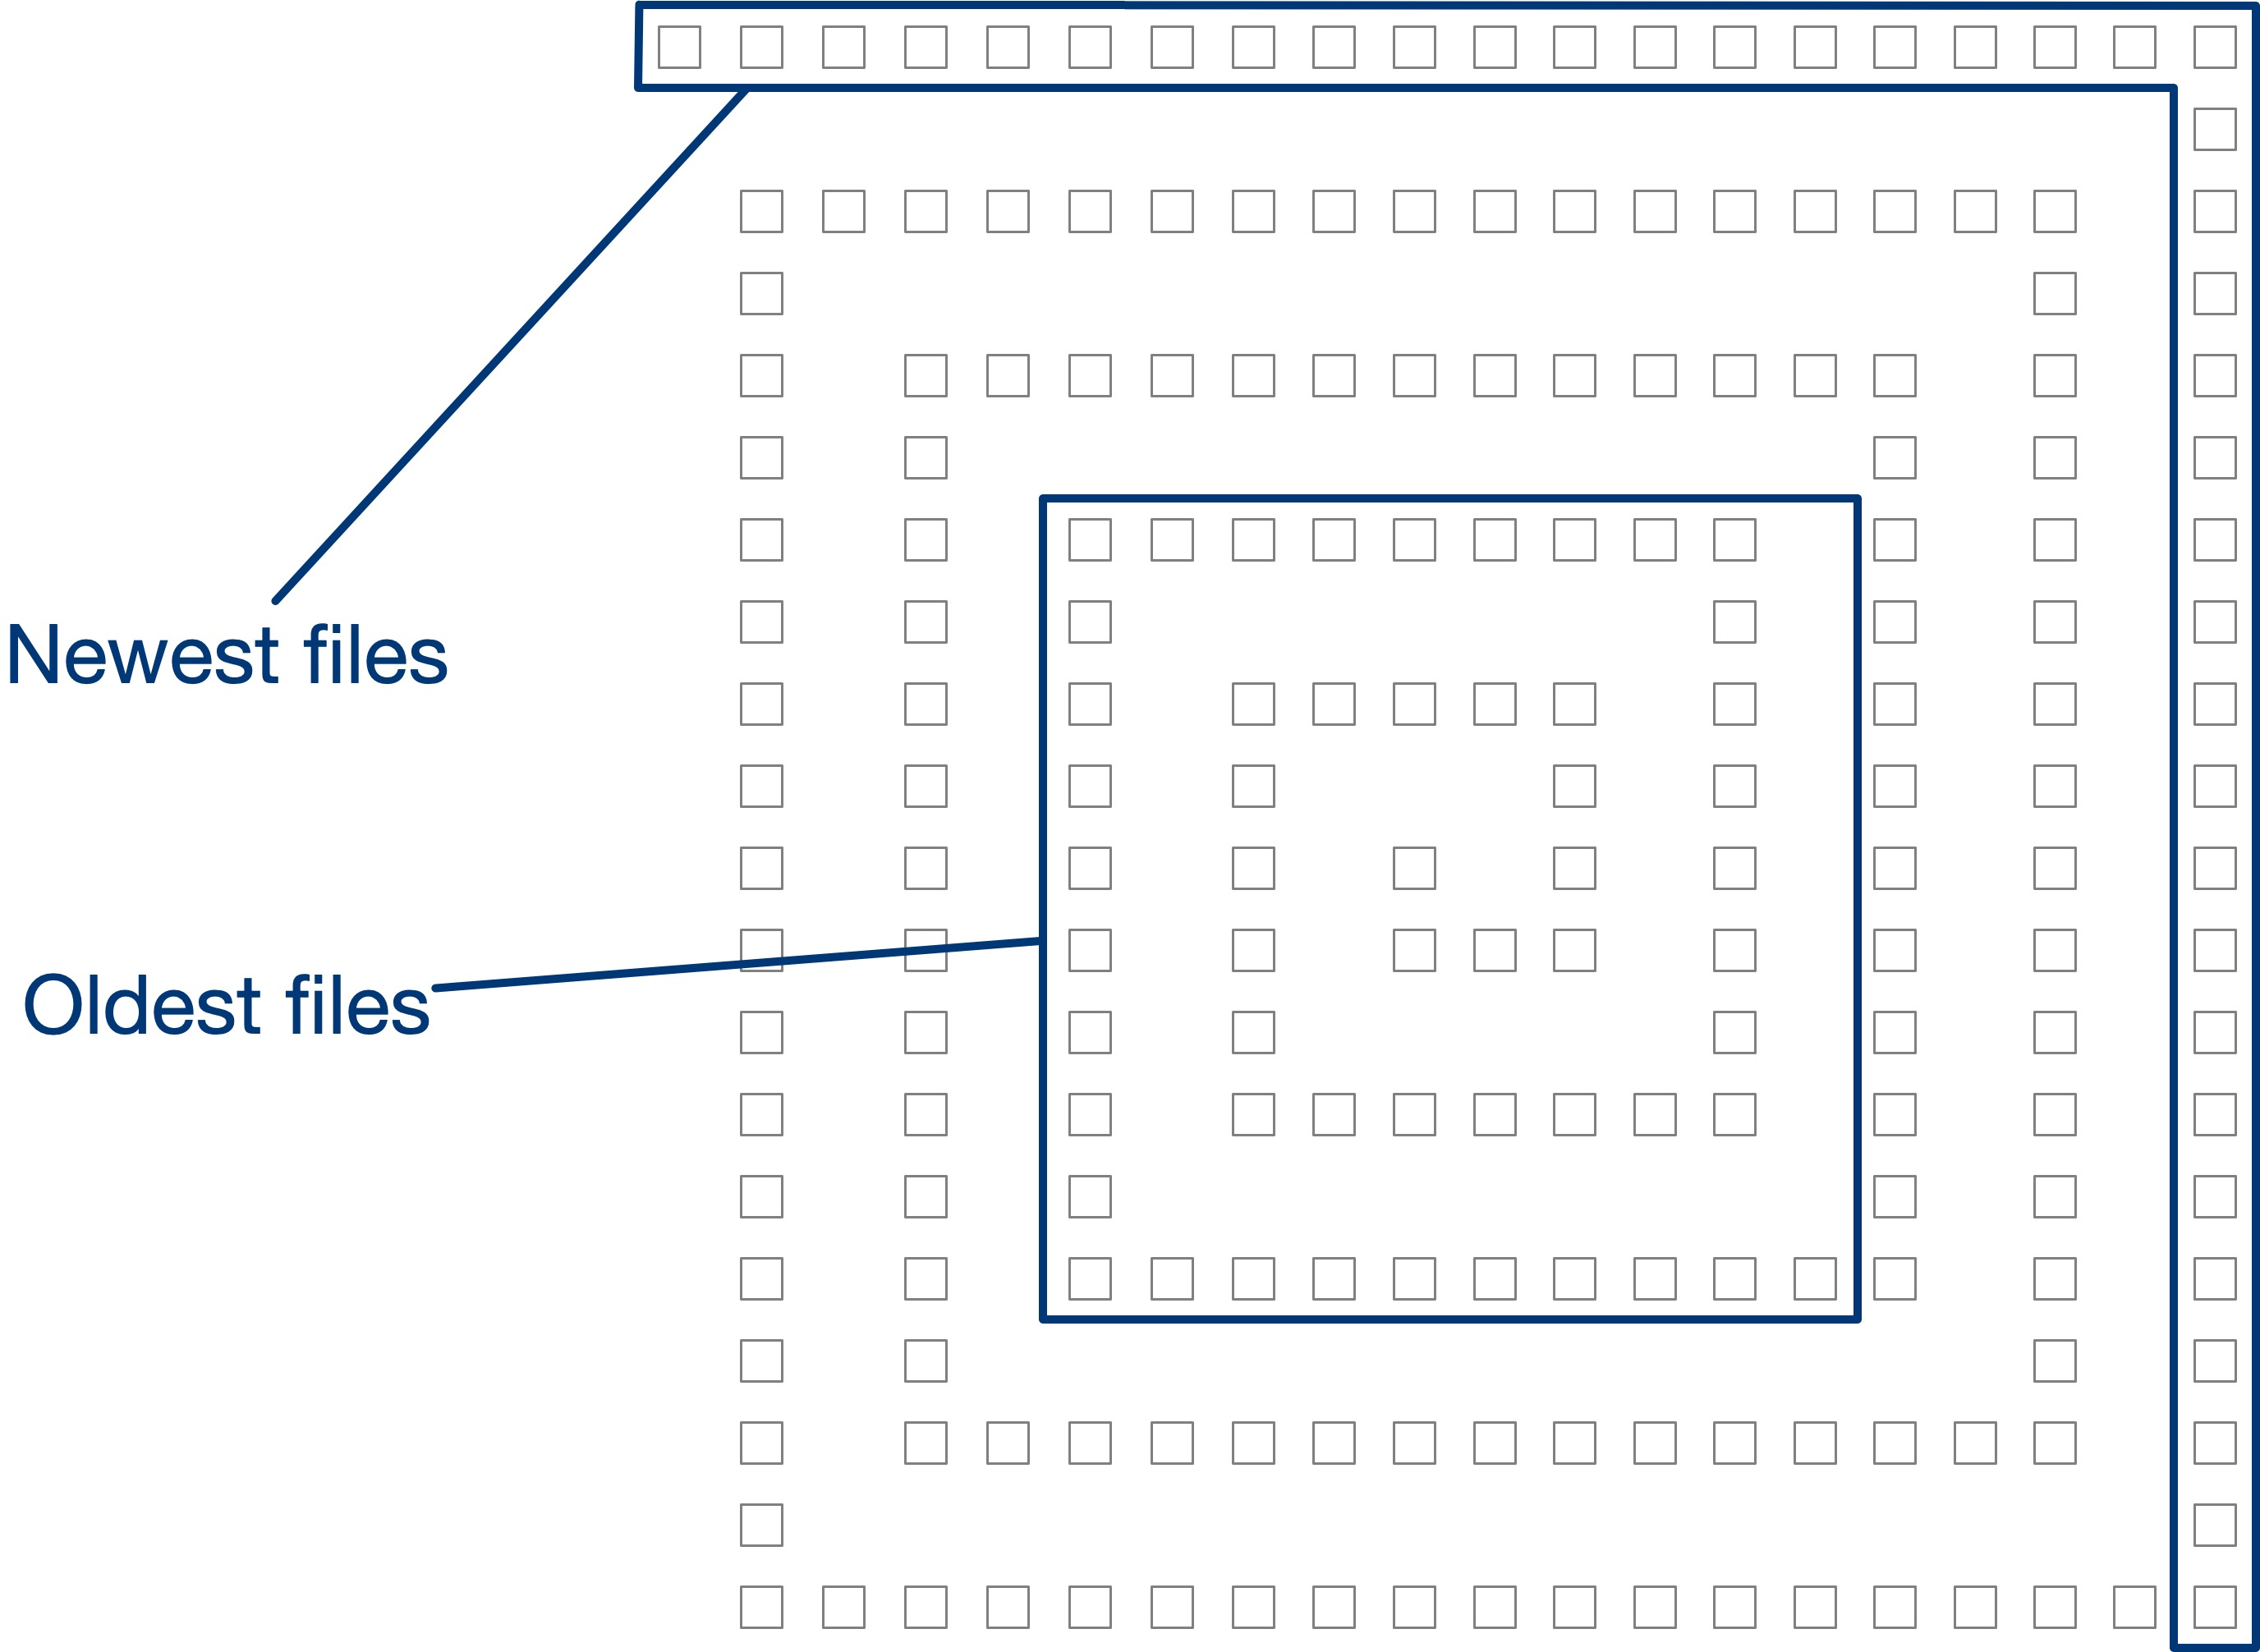
\includegraphics[width=\textwidth]{SpiralLayout.jpg}
    \caption{Outward spiral layout}
    \label{fig:layout}
\end{figure}

\subsection*{Color}

As we said, synesthesia occurs when we experience an involuntary stimulation of a cognitive path during the stimulation of another sense. Here we present how we used color to trigger the action made on a file automatically and how much time has passed since the action was made. 
As a result, we decided to map each git action with a color. \autoref{fig:ColorAssociation} shows how we mapped them in our approach. However, since each person has their own perception and way to reason, this mapping must be customizable by the user. Consequently, another property that a ViewFigure holds is \textit{color}.

In addition to the color, each ViewFigure has another property: the \textit{age}. We define the age of a file as the amount of time elapsed between the last action made on a file. Also there we defined two strategies to compute the age of an entity:

\begin{itemize}
    \item{Aging by commits}: the user specifies the number of commits \texttt{n} and then after \texttt{n} commits the age of a file is incremented by one. 
    \item{Aging by timestamp}:  the user specifies a timestamp window \texttt{ts} and then after \texttt{ts} seconds the age of a file is incremented by one.
\end{itemize}

When an action is made on a file its age is set to zero. 

The user also specifies the maximum age. When it is reached the color of the entity must be equal to the \texttt{base color}, chosen by the user. 
We initially set the base color equal to grey. \autoref{fig:Aging} shows how aging works with a file whose last action was an ADD and the maximum age is 10. 

All the files shared the same criteria to compute the age. The main purpose of the aging is to immediately distinguish files modified recently from files modified in past AnimationFrames.

\begin{figure}
    \center
    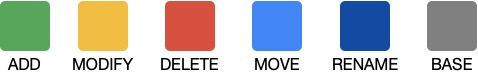
\includegraphics[width=0.\textwidth]{ColorMapping.jpg}
    \caption{Mapped colors to git actions}
    \label{fig:ColorAssociation}
\end{figure}


\begin{figure}
    \center
    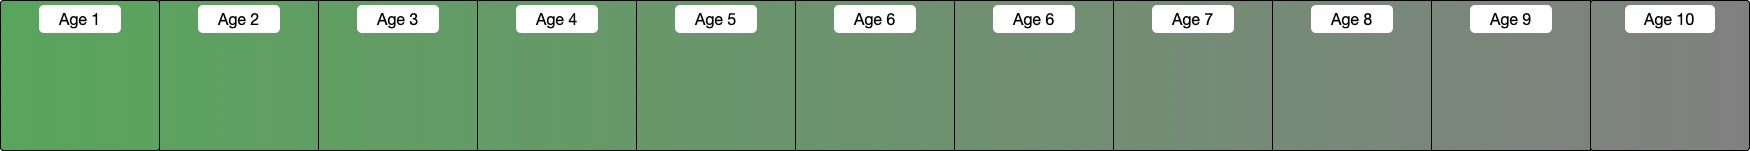
\includegraphics[width=\textwidth]{Aging.jpg}
    \caption{Aging process of an entity whose last action was an ADD and the maximum age is 10. }
    \label{fig:Aging}
\end{figure}



\subsection*{Shape and opacity}
To easily distinguish the type of the files, we added two properties to a ViewFigure: \textit{shape} and \textit{opacity}. 
In this way, the user can immediately understand the file type by looking at its shape. How FileTypes should be mapped to shapes must be part of the view specification because each engine works with different components. 

Moreover, we added the opacity to allow the highlight of a FileType over the others. 

\subsection*{Height}
The last information that we want to represent is the value of a metric. Since SYN has an extensible set of metrics, we decided to give the user the freedom to decide which metric should be used to represent the height of a file and how this height must be computed. 
To do that, we defined a mapper: a function that takes as input a metric and returns a double representing the ViewFigure height. The metric used by this mapper is the metric obtained from each file during the analysis. The set of mapper functions is extensible by the user. \bigbreak
This information is given to the render process through the \textit{height} property of a ViewFigure.

According to the mapping that we have presented so far, depicted in \autoref{fig:ApproachMapping}, the creation date of a file is mapped to the position of a ViewFigure, and the last action made on a file determines the color and the age of an entity, a chosen metric is used to compute the rendered height of the ViewFigure and finally, the type of the file is used to establish its shape and opacity. 

% \begin{itemize}
%     \item \textbf{Color}: to describe actions made on an entity (ADD, MODIFY, RENAME, MOVE, DELETE). 
%     \item \textbf{Shape}: to describe the type of the file. 
%     \item \textbf{Height}: to describe the value of a metric. The choiche of the metric is up to the user because it changes from project to project. 
% \end{itemize}

\begin{figure}
    \center
    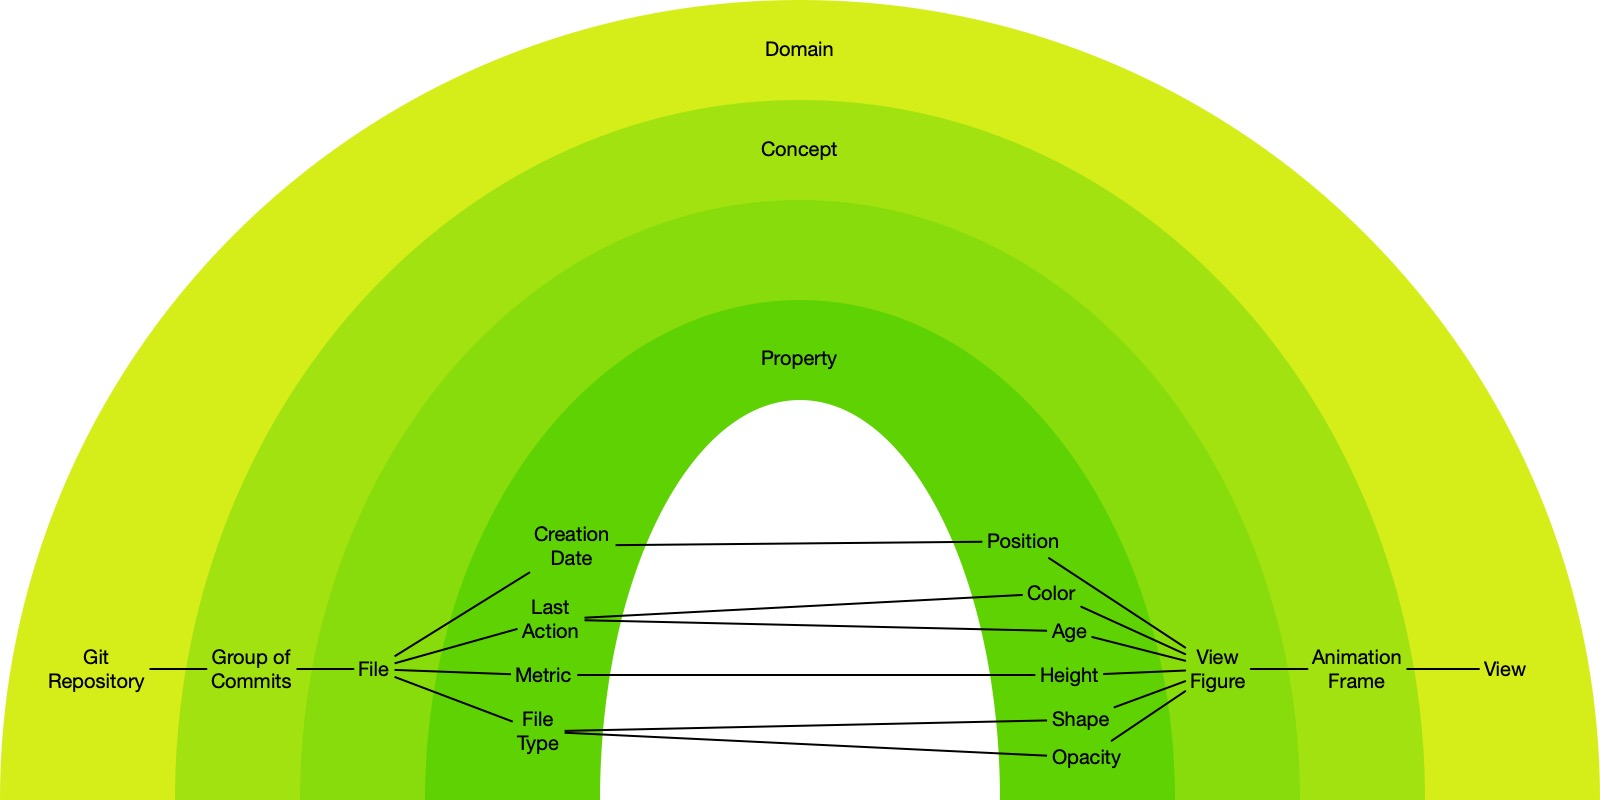
\includegraphics[width=\textwidth]{ApproachMapping.jpg}
    \caption{How properties are mapped in our approach}
    \label{fig:ApproachMapping}
\end{figure}



\section{Evolution Auralization}
\label{sec:audioApproach}
Displaying lots of information on the screen might not be an efficient way to gather crucial information about the evolution of software. Our approach provides an auditorial representation of an AnimationFrame to support its understanding task. The goal is to transmit hidden information such as the number of files added or removed in an AnimationFrame through audio notes. 

Music theory defines many concepts to study which aural phenomenons compose music. Examples are the Beats Per Minute (BPM), the pitch, or the note. We used them as a starting point to compose a sound for each AnimationFrame. In particular, in our approach, the following audio concepts are involved:
\begin{itemize}
    \item Tempo: indicates the speed of a musical composition. It is measured in BPM and sets the rhythm of a song. 
    \item Measure: a single unit of time featuring a specific number of beats. 
	\item Note's pitch: the quality that makes it possible to judge sounds as "higher" and "lower" in a sense associated with musical melodies.
	\item Amplitude: the size of the vibration of a note. It determines how loud a note is.
\end{itemize}

As Vickerts \cite{Vickers2004} stated, an orchestral model is needed to enable engineers to distinguish between different activities on the code. Following this idea, we decided to compose an auditorial portrayal of an  AnimationFrame mapping metrics to distinguishable sounds. Many intrinsic metrics could be extracted from an AnimationFrame. We focused our attention only on metrics extracted from git data:
\begin{itemize}
    \item total number of commits
    \item the number of files added/removed/modified/renamed or moved
    \item total number of lines added/removed
\end{itemize}
This set can be easily extended depending on the goal of the melody. For example, we can create a new metric to play how many java files were added. The implementation must be done with a tool that provides synthesizers to create different sounds for each metric. A synthesizer is a component that generates audio signals. For example, a synthesizer can play the sound of a guitar, whereas another can play the sound of a piano. The idea is to allow the user to understand what is happening on the displayed AnimationFrame by recognizing the instrument through the sound. 

We defined criteria on how notes should be played. The output of this approach is a piece of music representing a system's whole evolution. The evolution of a system was depicted as a sequence of AnimationFrames. Therefore, we decided to map a measure to each AnimationFrame. As a consequence, the total length of the evolution visualization depends upon the tempo and the size of a measure. 
For example, if we display a view with 60 AnimationFrames, each one mapped to a measure long of four beats playing at 60 BPM, to visualize the view, we need four minutes ($240$ beats played at $60$ BPM). As well as notes, also the value of BPM depends upon a metric. Therefore, some visualizations might suffer from this approach because, with a high BPM value, the time between two AnimationFrames might not be sufficient. To overcome this issue, a fixed interval between such as one second or two AnimationFrames can be set. Consequently, the same view of 60 AnimationFrames now needs one minute to be played. Within each second, for each chosen metric, we play sounds with an amplitude and a speed that depends upon the metric value. 

To summarize, in our auditorial approach, we support the visualization of a project's view with a musical representation of each AnimationFrames. Metrics collected during the analysis are used in an orchestral composition to control the tempo, the note, and the amplitude. An exemplary implementation should provide a wide range of synthesizers to play different sounds representing adopted metrics. We can choose to play one AnimationFrame every second or map it to a measure. 










